\section{Event selection}
\label{sec:selection}
This analysis is based on the final state $hh \to \bbWW \to l \nu q\bar{q} b\bar{b}$. The semileptonic final state was chosen as a compromise between an acceptable branching fraction and the reduction of multi-jet background since the fully hadronic channel suffers from large multi-jet backgrounds while the fully leptonic channel suffers from the low branching fraction $WW^* \to l \nu l \nu$. %Since  $t \bar{t} \to WWb\bar{b}$ is the dominant background in both the semi- and fully leptonic channels, selecting the di-leptonic channel does not reduce the top background it merely results in a reduction of the signal yield.
The final state is therefore characterized by the presence of one lepton, two light jets, two $b$-jets, and \met from the escaping neutrino.

Correctly identifying the pair of light jets produced by the hadronic $W$ decay is important in the event reconstruction both for a correct reconstruction of the $W$ and also for the higgs boson decaying to $WW^*$ since the hadronic $W$ information is also used to solve for the $z$ component of the neutrino momentum. There is an additional complication due to the fact that one of the $W$ bosons is off-shell, so there is no $W$ mass constraint for one of the $W$ bosons. This section details the stages of the event reconstruction and the final selection which defines the signal region. Control regions used to the background modeling are defined in Section~\ref{sec:plots_cut_flow}. The signal regions are blinded (no data is shown in the signal region) since the final analysis has not yet been approved by the ATLAS collaboration. The evaluation of the background modeling and the expected sensitivity of the analysis are presented.

\subsection{Trigger requirement}
Events are selected using the un-prescaled single lepton triggers. The list of triggers used in this analysis is shown in Table~\ref{tab:triggers}. Events are selected with a logical OR between the triggers listed in Table~\ref{tab:triggers}.
\begin{table}[htbp!]
\begin{center}
 \begin{tabular}{|c|c|}
  \hline
  Dataset & Trigger items \\
  \hline
  \multirow{2}{*}{2015} & mu20\_iloose\_L1MU15  \\
    & mu50  \\
    & e24\_lhmedium\_L1EM18VH (MC)  \\
    & e24\_lhmedium\_L1EM20VH (data)  \\
    & e60\_lhmedium  \\
    & e120\_lhloose  \\
  \hline
  \multirow{8}{*}{2016 - Period A} & mu24\_iloose\_L1MU15 (MC)  \\
    & mu24\_iloose (data)  \\
    & mu40  \\
    & e26\_lhtight\_nod0\_ivarloose  \\
    & e60\_lhmedium\_nod0  \\
    & e60\_medium  \\
    & e140\_lhloose\_nod0  \\
    & e300\_etcut  \\
  \hline
  \multirow{7}{*}{2016 - Period B-D3} & mu24\_ivarmedium  \\
    & mu50  \\
    & e26\_lhtight\_nod0\_ivarloose  \\
    & e60\_lhmedium\_nod0  \\
    & e60\_lhmedium  \\
    & e140\_lhloose\_nod0  \\
    & e300\_etcut  \\
  \hline
  \multirow{7}{*}{2016 - Period D4-E3} & mu26\_ivarmedium  \\
   & mu50  \\
   & e26\_lhtight\_nod0\_ivarloose  \\
   & e60\_lhmedium\_nod0  \\
   & e60\_lhmedium \\
   & e140\_lhloose\_nod0  \\
   & e300\_etcut  \\
  \hline
  \multirow{7}{*}{2016 - Period $\ge$ F} & mu26\_ivarmedium   \\
   & mu50  \\
   & e26\_lhtight\_nod0\_ivarloose  \\
   & e60\_lhmedium\_nod0  \\
   & e60\_lhmedium  \\
   & e140\_lhloose\_nod0  \\
   & e300\_etcut  \\
  \hline
 \end{tabular}
\end{center}
\caption{Summary of trigger items used for 2015 and 2016 data. For 2016 data, different triggers were used for different data run periods. 
All triggers are un-prescaled.}
\label{tab:triggers}
\end{table}

\subsection{Event pre-selection}
The following selection criteria are applied before any cuts are applied on the physics objects in an event
\begin{itemize}
\item In order to assure good data quality, events with bad detector conditions, namely where large part of the detectors were missing from data acquisition due to problems during a run, or when the performance of the detectors were affected by large noise, have been rejected from the data analysis. Incomplete events or events with bad detector information are rejected. 
\item The presence of at least one primary vertex with at least two tracks is required. Among all primary vertices, the vertex with the highest $\sum p_{{\rm T,trk}}^{2}$, where $p_{{\rm T,trk}}$ is the transverse momentum of tracks associated with the vertex, is retained as the primary interaction vertex.
\item The presence of at least one signal electron ($e$) or signal muon ($\mu$) is required. The definitions for signal electrons and muons are given in Sec.~\ref{sec:electron13TeV} and Sec.~\ref{sec:muon13TeV} respectively. The signal lepton must be trigger matched to the corresponding HLT object which fires the trigger.
\item There must be at least four jets surviving object selection of which two and only two are $b$-tagged.
\end{itemize}


\subsection{Event Reconstruction}
%%The final state of our signal consists of one charged lepton, one neutrino, and four quarks, 
%%two being $b$-quraks. Hence the detector signature consists of one charged lepton, missing 
%%transverse momentum, and four or more jets of which two are $b$ jets from the $h$ decay while 
%%the other two are light jets from the hadronic decay of the $W$ boson. 
Events are reconstructed by first requiring exactly two $b$-tag jets and either two or three light jets. In events with three light jets, the pair with the lowest $\Delta R$ between them are selected as $W$ jet candidates. This procedure yields the correct jet assignment in 70\% of the cases where the hadronic daughters of the $W$ boson can be correctly matched to reconstructed jets.% as described in Appendix~\ref{app:jetTruthStudies}.

The event kinematics of the $h \to WW^* \to l \nu qq$ topology can be fully reconstructed since the only unknown component of the final state objects is the neutrino momentum along the beam axis, $p_z$. Imposing the relation
\begin{equation}
\label{eq:mh}
m_h^2 = (p^l + p^{\nu} + p^{j1} + p^{j2})^2
\end{equation}
where $p^i$ is the four-momenta of particle $i$, the neutrino $p_z$ can be reconstructed using 
\[
p_E^{\nu} = E^{\nu} = \sqrt{\pt^2 + p_z^2}, \quad p_x^{\nu} = \pt\cos(\phi), \quad p_y^{\nu} = \pt\sin(\phi)
\]
where $\phi$ is the azimuthal angle of the $\met$, $E^{\nu}$ the neutrino energy, and $p_{x}$ and $p_{y}$ are the two transverse spatial components of the neutrino momentum. Eq. \ref{eq:mh} is a quadratic expression in $p_z$, so it can have either two real, one real, or two complex solutions. In the last case, only the real part of the complex solution is taken into account leaving a single value of $p_z$. In the first case, the solution with the neutrino direction closest to the charged lepton is retained. Following this algorithm results in choosing the correct solution in approximately 60\% of the selected events.%(see Appendix~\ref{app:nupz_studies}).

\subsection{$b\bar{b}\tautau$ analysis overlap removal}
In order to remove overlap with an ATLAS search for dihiggs production in the $b\bar{b}\tautau$ final state, events are rejected which contain at least one hadronic $\tau$ candidate. This orthogonality between analyses is useful for future efforts to combine the results of multiple dihiggs searches in order place more stringent limits than can be produced by a search in any single final state. Events containing hadronic tau candidates that fulfill the following requirements
\begin{itemize}
\item have $p_T > 20$ GeV and $|\eta| < 2.5$
\item are reconstructed with one or three prongs
\item possess unit charge
\item pass a medium $\tau$ identification working point
\end{itemize}
are rejected. This rejection causes a signal efficiency loss of about 3\%.

\subsection{Kinematic selection}
\label{subsec:kincuts}
Since one of the largest backgrounds of this search comes from semileptonic \ttbar decays, kinematic cuts placed on selected events designed to suppress the \ttbar background while keeping a large signal efficiency.  A schematic view of $hh \to \bbWW$ and the $\ttbar \to WbWb$ event topologies is shown in Figure \ref{fig:cartoon}.
\begin{figure}
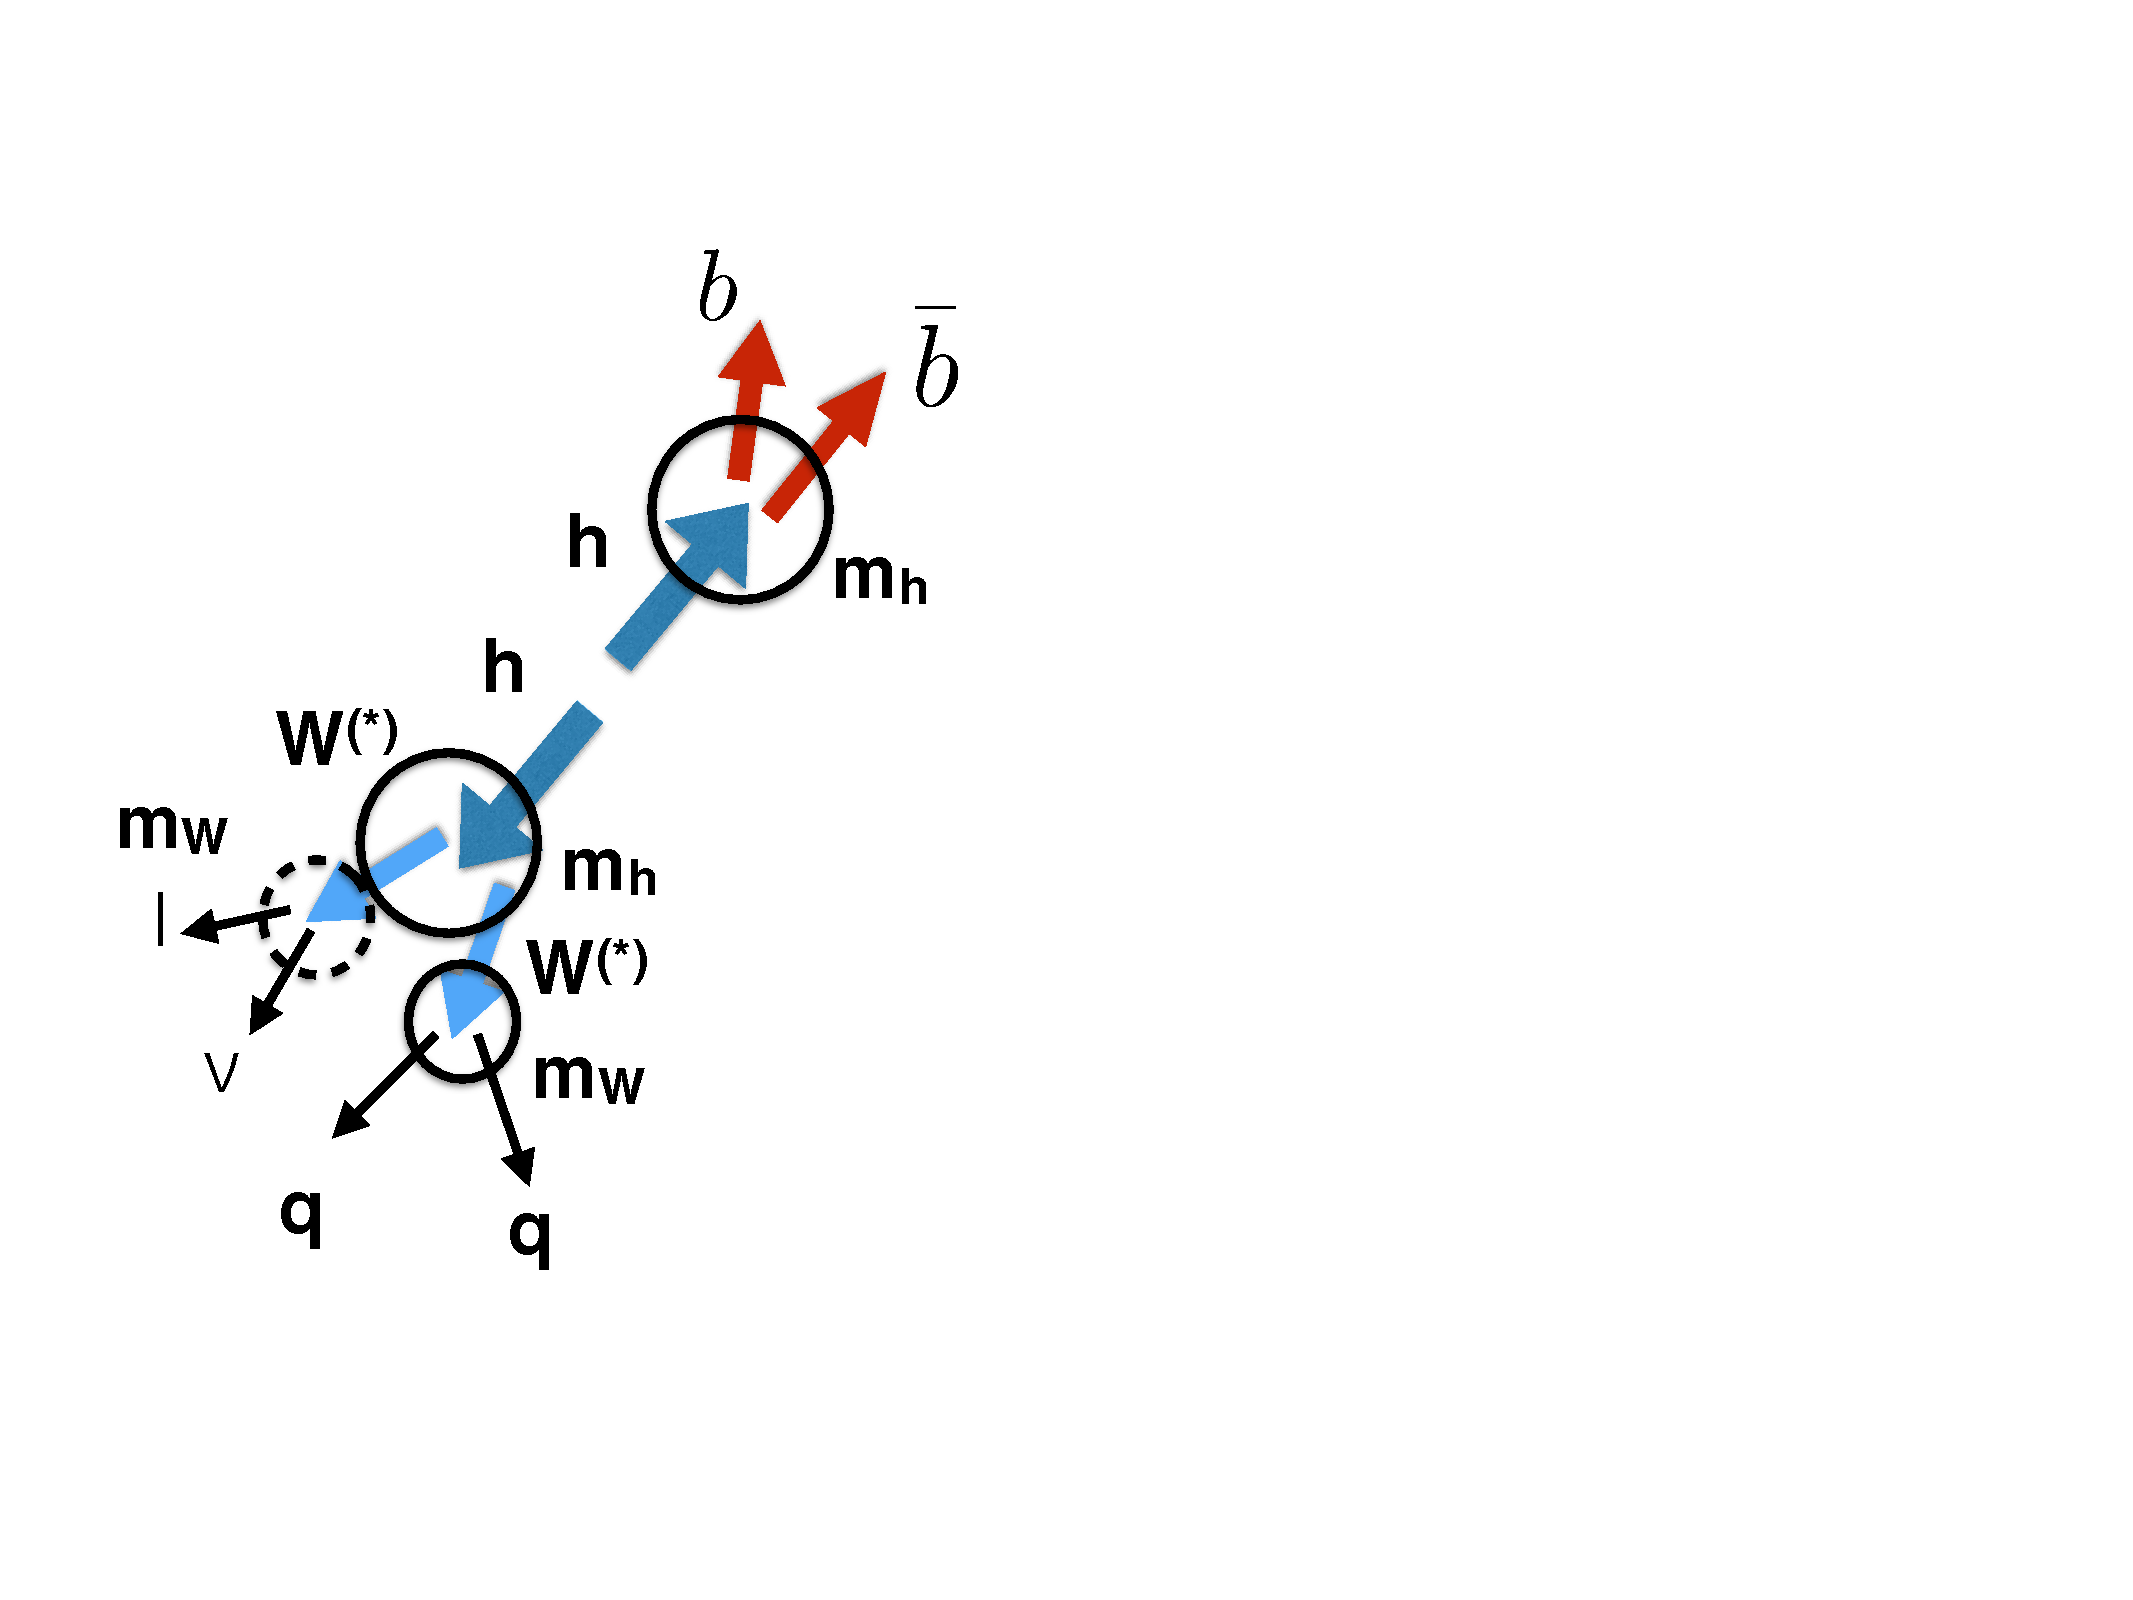
\includegraphics[width=0.5\textwidth]{chapters/dihiggs2/figures/cartoon_hh.pdf}
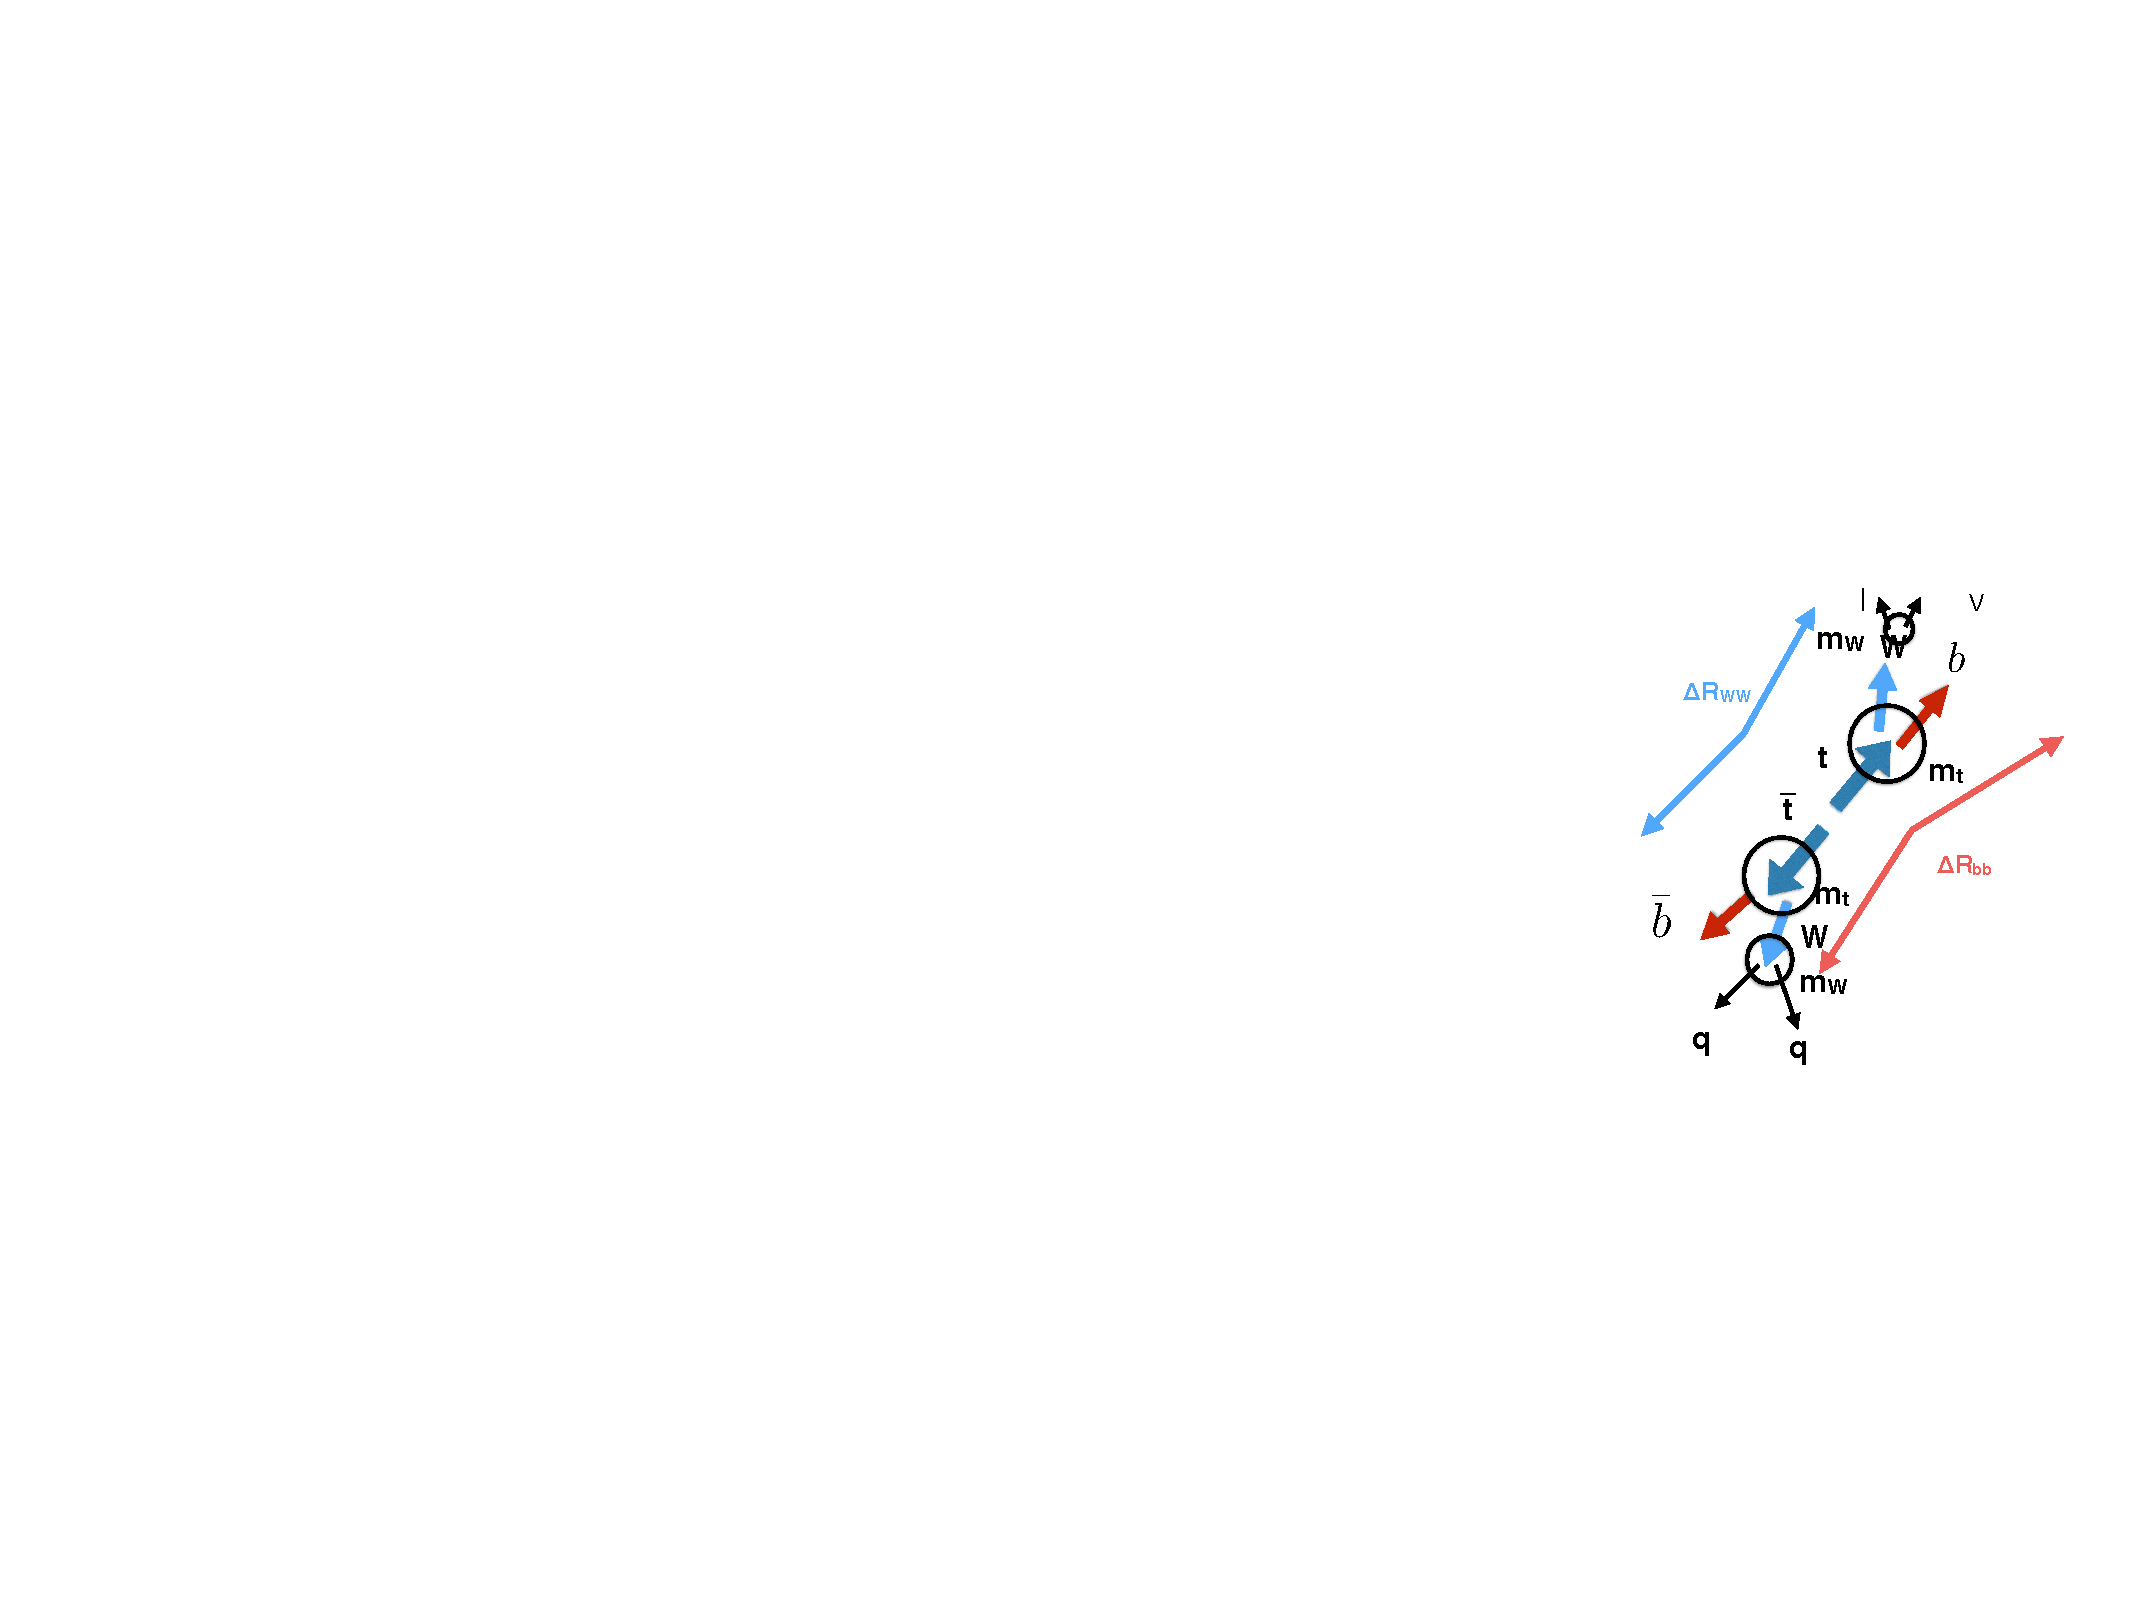
\includegraphics[width=0.5\textwidth]{chapters/dihiggs2/figures/cartoon_tt.pdf}
\caption{Schematic view of a $hh \to WWbb$ event compared to a $t\bar{t} \to WWbb$ event.} 
\label{fig:cartoon}
\end{figure}
While semileptonic \ttbar and $hh\rightarrow bbWW$ decays are both characterized by the presence two $b$-jets and two $W$ bosons, the $\Delta R$ separation between the two $b$-jets and the two $W$ bosons is much larger for \ttbar events than for dihiggs events. The mass spectrum of the $b\bar{b}$ pair can also be used as a discriminant since \mbb should be close to $m_h$ in dihiggs events while there is no resonant value for \ttbar. The full set of variables used in the event selection variables are given by
\begin{itemize}
\item the $p_T$ of the $b \bar{b}$ pair (\ptbb)
\item the $\Delta R$ of the $b \bar{b}$ pair (\drbb)
\item the $p_T$ of the $WW$ pair ($p_T^{WW}$)
\item the $\Delta R$ of the $WW$ pair ($\Delta R^{WW}$)
\item the mass of the $WW$ system computed using the calculated neutrino longitudinal momentum ($m_{h}$). This value is exactly equal to $m_h$ if a real solution is found, it is larger if no real solution is found
\item the invariant mass of the dihiggs boson system ($m_{hh}$) 
\item the invariant mass of the 2 b-jets boson system (\mbb) 
\end{itemize}

% START HERE
\subsection{Signal region definitions}
\label{subsec:SR}
The cuts of the selection were optimized by maximizing the Poisson significance at the end of the selection. A two step procedure has been implemented in order to final the optimal set of selection cuts. In the first step each cut is individually optimized. In the second step, all cuts are set to their optimal value and cuts are varied one by one to test the stability of the optimal point since correlations among the variables could alter the results obtained in the first step. %The Poisson significance formula depends on the absolute yield of expected signal and background events. 
The \ttbar background was normalized to data in the region $\mbb < 100$ GeV and $\mbb > 140$ GeV (orthogonal to the final signal region) during the optimization. 

Three different optimizations were produced using i) a non-resonant dihiggs signal, ii) a heavy Higgs with $m_H = 700$ GeV (low-mass), and iii) a resonant heavy Higgs with $m_H = 2000$ GeV (high mass). The resonant signals is normalized to the Run-1 upper limit scaled by the $13/8$ TeV cross section ratio expected from the PDF luminosity scale of a narrow resonance of that mass. The non-resonant signal is normalized to the Standard Model expectation. The results of the optimizations for the three reference signal hypotheses are summarized in Table~\ref{tab:sig_reg_summary}.
%%%%%%%%%%%%%%
\begin{table}
\label{tab:sig_reg_summary}
\begin{center}
\begin{tabular}{|c|c|c|c|c|c}
\hline 
Variable 				& non-resonant 	 	& low-mass 		& high-mass\\
\hline
$\met$ (GeV)				& $> 25 $		& $> 25 $		& $> 25 $\\
$m_{WW}$ (GeV)   			& $<130$ 		&$<130$ 		& no-cut \\
$p_{\rm T}^{bb}$ (GeV) 			& $>230$ 		& $>150$ 		&$>350$\\
  \drbb  				& $<1.2$ 	 	& $<1.1$ 		& no-cut  \\
$p_{\rm T}^{WW}$ (GeV) 			& no-cut	 	& no-cut   		& $>360$ \\
$\Delta R_{WW}$  			& $<1.1$ 		& $<0.9$ 		& $<2.0$ \\
$m_{hh}$ (GeV)  			& no-cut 		& see Table~\ref{tab:mhh_sig_cuts} 	& see Table ~\ref{tab:mhh_sig_cuts}\\
\mbb (GeV)   				& 105-135 	 	& 105-135 	& 105-135\\
\hline
\end{tabular}
\end{center}
\caption{Event selections for the non-resonant, low, and high mass selections. $m_{hh}$ is not applied for non-resonant signal, and for resonant signals $m_{hh}$ depends on the mass.} \end{table}
%%%%%%%%%%%%%%%
In the low and high mass selections, a $m_{hh}$ dependent cut is applied. The window edges are obtained by maximizing the expected signal significance. The $m_{hh}$ interval used for each mass point is shown in Table~\ref{tab:mhh_sig_cuts}. 

\begin{table}
\label{tab:mhh_sig_cuts}
\begin{center}
\begin{tabular}{c|c|c}
  Signal Mass & low-mass & high-mass\\
\hline
500 & $[ 450, 550] $   & $[ NA ] $ \\
600 & $[ 520, 680] $ & $[ NA ] $\\ 
700 & $[ 630, 770] $ & $[ 480, 920 ] $\\ 
750 & $[ 680, 820] $ & $[ 660, 840] $\\ 
800 & $[ 720, 880] $ & $[ 730, 870] $\\ 
900 & $[ 800, 1000] $ & $[ 750, 1050] $\\ 
1000 & $[ 940, 1060] $ & $[ 870, 1130] $\\ 
1100 & $[ 960, 1240] $ & $[ 880, 1320] $\\ 
1200 & $[ 1090, 1310] $ & $[ 1030, 1370] $\\ 
1300 & $[ 1180, 1420] $ & $[ 1160, 1440] $\\ 
1400 & $[ 1200, 1600] $ & $[ 1210, 1590] $\\ 
1500 & $[ 1260, 1740] $ & $[ 1320, 1680] $\\ 
1600 & $[ 1370, 1830] $ & $[ 1380, 1820] $\\ 
1800 & $[ 1560, 2040] $ & $[ 1620, 1980] $\\ 
2000 & $[ 1770, 2230] $ & $[ 1770, 2230] $\\ 
2250 & $[ 2040, 2490] $ & $[ 2040, 2460] $\\ 
2500 & $[ 2260, 2740] $ & $[ 2260, 2740] $\\ 
2750 & $[ 2520, 2980] $ & $[ 2550, 2950] $\\ 
3000 & $[ 2770, 3230] $ & $[ 2790, 3210] $\\  
\hline
\end{tabular}
\end{center}
\caption{$m_{hh}$ selection for the low mass and high mass searches corresponding to best discovery significance.} 
\end{table}
